% 尘埃云的能动张量

\pentry{动力学假设\upref{SRDyn},张量\upref{Tensor}}

%未完成
%应阐释:能动张量可以看成什么到什么的线性映射
%任意尘埃云的能动张量是什么

\subsection{均匀等速尘埃云的动量通量}

\subsubsection{均匀等速尘埃云}

在任意参考系中,空间中分布若干质点.这些质点的集合,被称为一片\textbf{尘埃云(dust)},各质点被称为\textbf{尘埃粒子}.如果在某个参考系中,一片尘埃云的各质点都保持静止,那么我们称这个参考系是尘埃云的\textbf{自身系},称尘埃云为\textbf{等速尘埃云},因为这意味着在其它参考系中,尘埃粒子的速度都会是相同的.如果在某个参考系中,尘埃粒子的质量相同、在空间中均匀分布,那么我们称这片尘埃云是\textbf{均匀的}.

任何一片\textbf{均匀尘埃云},都可以看成是许多\textbf{均匀等速尘埃云}的叠加,只要把属于各个速度的尘埃粒子分别拿出来构成尘埃云即可.而任何一片尘埃云,也可以看成是局部均匀的.因此,研究均匀等速尘埃云的性质最为容易,也可以方便地拓展到任意尘埃云的性质中.

\subsubsection{尘埃云数量通量密度}

假设空间中有一片均匀等速尘埃云,在其自身系中各点的粒子数量密度都是$n$,其中$n$是一个实数.也就是说,在尘埃云的自身系中,在任何体积$V$中,尘埃粒子的数量都是$nV$.

取$K_1$参考系作为观察者,设观察者认为尘埃云的速度是$\bvec{v}=(v_x, v_y, v_z)^T$.由于尺缩效应,在$K_1$中,空间各点尘埃粒子的数量密度变为$n/\sqrt{1-v^2}$.

\begin{figure}[ht]
\centering
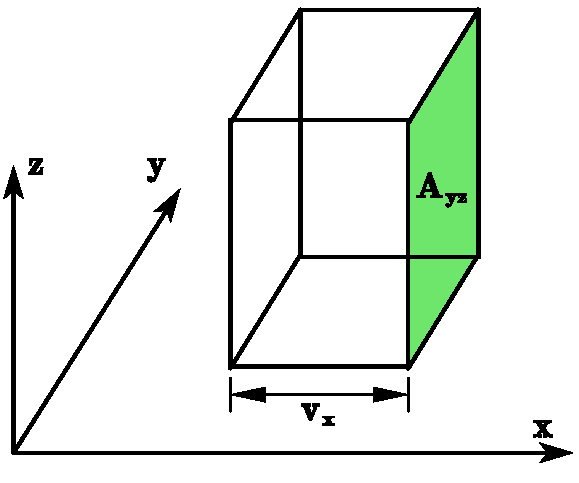
\includegraphics[width=10cm]{./figures/SRFld_1.pdf}
\caption{粒子数量通量示意图.绿色面表示计算粒子数量通量的参考平面$A_{yz}$;一个粒子在单位时间后通过这个平面,当且仅当这个粒子现在正在图示体积内.该体积的四条红色边和尘埃云的速度方向平行,而左右两个平面之间的距离是$v_x$,故体积为$A_{yz}\cdot v_x$.} \label{SRFld_fig1}
\end{figure}

固定$x$坐标,取此处$y-z$平面上的一个单位面积$A_{yz}$.如所示,在单位时间内,通过$A_{yz}$的是体积$A_{yz}\cdot v_x=v_x$内的粒子,数量是
\begin{equation}
\frac{n}{\sqrt{1-v^2}}\cdot v_x=\frac{nv_x}{\sqrt{1-v^2}}
\end{equation}

类似地,用$i, j, k$代表任意的字母$x, y, z$,那么对于固定的$i$坐标,单位时间内通过$j-k$平面上的单位面积的粒子数量是$nv_i/\sqrt{1-v^2}$.通过一个平面的尘埃粒子数量,称为尘埃云通过这个平面的数量通量;而当所通过平面的面积是单位面积时,数量通量也可以称为数量密度的通量,或者数量通量的密度.

总结下来,如果取所考察平面的面积向量为$\bvec{S}$,那么对于上述均匀等速尘埃云,单位时间内通过这个平面的粒子数量是$\frac{n}{\sqrt{1-v^2}}\abs{\bvec{v}\cdot\bvec{S}}$.

\subsubsection{尘埃云动量通量密度}

尘埃云设定同上,并假设每个尘埃云粒子的质量是$m$,那么它在$K_1$中的动量是$m/\sqrt{1-v^2}$.结合数量通量密度可知,在单位时间内通过面积$\bvec{S}$的尘埃云动量是
\begin{equation}
\frac{n}{\sqrt{1-v^2}}\abs{\bvec{v}\cdot\bvec{S}}\cdot\frac{m}{\sqrt{1-v^2}}\bvec{v}=\frac{nm\bvec{v}}{1-v^2}\abs{\bvec{v}\cdot\bvec{S}}=\frac{nm}{1-v^2}\abs{\bvec{v}\cdot\bvec{S}}\cdot\pmat{v_x\\v_y\\v_z}
\end{equation}

固定$x$坐标时,单位时间内通过单位面积的尘埃云动量的$y$分量就是
\begin{equation}
\frac{nm}{1-v^2}v_xv_y
\end{equation}

一般地,固定$i$坐标时,单位时间内通过单位面积的尘埃云动量的$j$分量就是
\begin{equation}\label{SRFld_eq1}
\frac{nm}{1-v^2}v_iv_j
\end{equation}

\subsection{四动量通量密度和能量-动量张量}

上面所讨论的动量通量密度,在四维闵可夫斯基空间中可以表示为穿过单位时间、单位$A_{yz}$面积的\textbf{三维“平面”}\footnote{多维几何学中,将$n$维空间中的一个$n-1$维子空间称为一个\textbf{超平面(hypersurface)},因此这里的三维平面,指的是四维空间中的三维超平面.}的世界线数量乘以各世界线代表的动量.

\autoref{SRFld_fig2} 是四维闵可夫斯基空间中的动量通量示意图,绿色的垂直线段表示单位时间长度里的单位面积 $A_{yz}$,相当于用一维线段表示了一个三维的体积;若干红色线段表示各尘埃粒子的世界线.动量通量密度,就是通过单位时间单位面积的世界线数量乘以各粒子的动量\footnote{这里有一个视错觉现象,即绿色线段看起来不是垂直的,而是微微倒向左边.}.

\begin{figure}[ht]
\centering
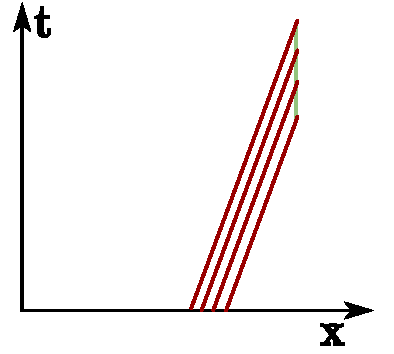
\includegraphics[width=6cm]{./figures/SRFld_2.pdf}
\caption{四维闵可夫斯基空间中的动量通量} \label{SRFld_fig2}
\end{figure}

既然都用到四维表示了,我们也可以把结论拓展到四动量,以及固定时间的情况.

\begin{figure}[ht]
\centering
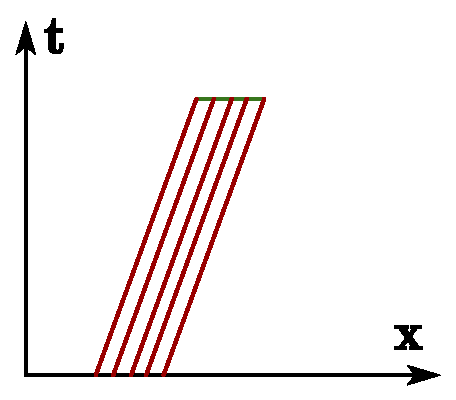
\includegraphics[width=6cm]{./figures/SRFld_3.pdf}
\caption{固定时间时,穿过单位三维空间超平面的世界线示意图.} \label{SRFld_fig3}
\end{figure}

如果设各尘埃粒子的四速度是$\bvec{U}=1/\sqrt{1-v^2}(1, v_x, v_y, v_z)^T$,可以定义一个矩阵$\bvec{M}$,其第$i$行$j$列的元素代表“固定$i$坐标时,单位时间内通过单位面积的尘埃云动量的$j$分量”,那么就有

\begin{equation}
\bvec{M}=\frac{nm}{1-v^2}\pmat{1&v_x&v_y&v_z\\v_x&v_x^2&v_xv_y&v_xv_z\\v_y&v_xv_y&v_y^2&v_yv_z\\v_z&v_xv_z&v_yv_z&v_z^2}=nm\cdot\bvec{U}\bvec{U}^T
\end{equation}

这里的$\bvec{U}$是一个列矩阵,也就是说,$\bvec{M}$是向量$n\bvec{U}$和$m\bvec{U}$的张量积.$\bvec{M}$因而是一个二阶张量,被称作\textbf{能量-动量张量}.




